\documentclass[tikz,border=8pt]{standalone}
\usepackage{lmodern}\usetikzlibrary{arrows.meta,positioning,fit,backgrounds}
\definecolor{aws}{HTML}{EAF2F8}\tikzset{actor/.style={draw,rounded corners,fill=black!5,minimum width=23mm,minimum height=10mm,align=center,font=\sffamily\scriptsize},aws/.style={actor,fill=aws},ext/.style={actor,fill=orange!12},edge/.style={-{Latex[length=1.6mm]},thick,font=\sffamily\tiny,align=center}}
\begin{document}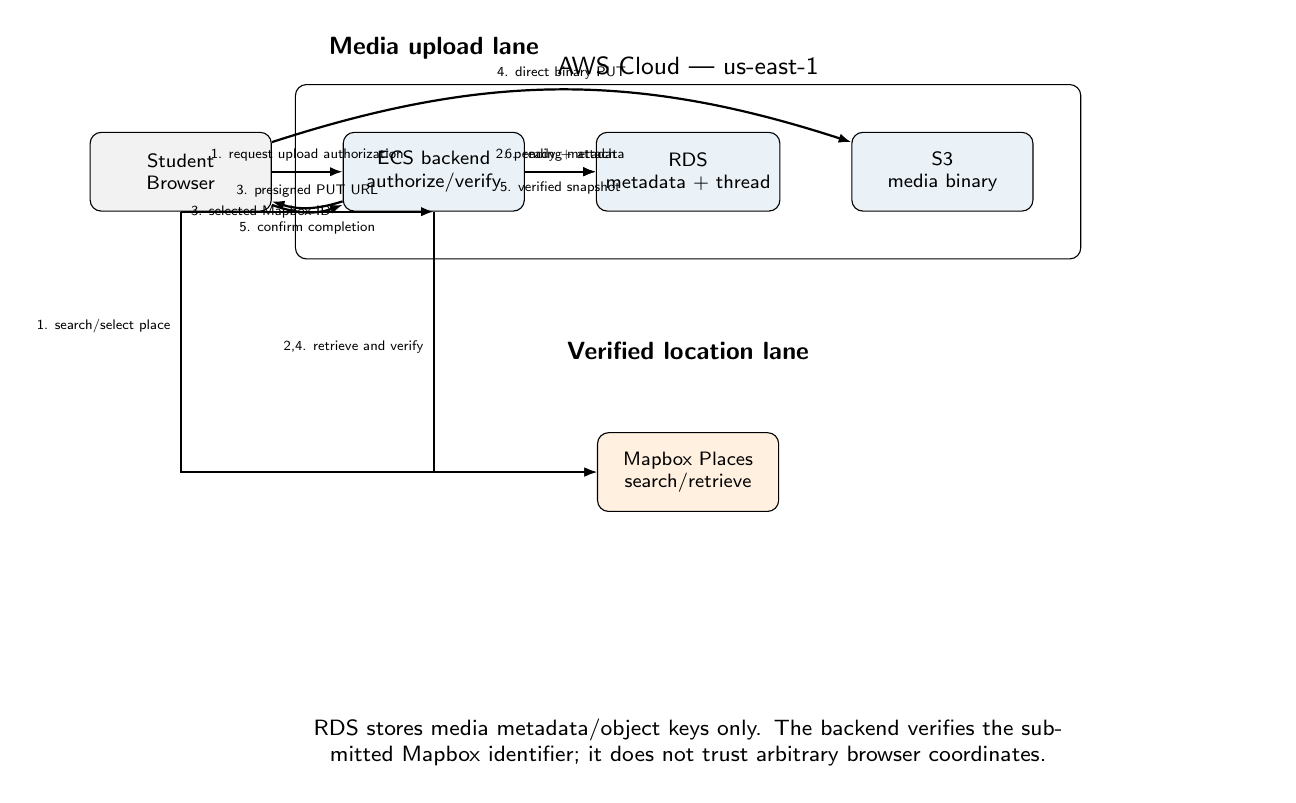
\begin{tikzpicture}[node distance=8mm and 9mm]
\node[actor] (student) {Student\\Browser};\node[aws,right=of student] (ecs) {ECS backend\\authorize/verify};\node[aws,right=of ecs] (rds) {RDS\\metadata + thread};\node[aws,right=of rds] (s3) {S3\\media binary};\node[ext,below=28mm of rds] (mapbox) {Mapbox Places\\search/retrieve};
\node[font=\sffamily\bfseries\small,above=8mm of ecs] {Media upload lane};
\draw[edge] (student) -- node[above]{1. request upload authorization} (ecs);\draw[edge] (ecs) -- node[above]{2. pending metadata} (rds);\draw[edge] (ecs) to[bend left=18] node[above]{3. presigned PUT URL} (student);\draw[edge] (student) to[bend left=18] node[above]{4. direct binary PUT} (s3);\draw[edge] (student) to[bend right=20] node[below]{5. confirm completion} (ecs);\draw[edge] (ecs) -- node[above]{6. ready + attach} (rds);
\node[font=\sffamily\bfseries\small,above=8mm of mapbox] {Verified location lane};
\draw[edge] (student.south) |- node[pos=.22,left]{1. search/select place} (mapbox.west);\draw[edge] (student.south) |- node[pos=.24,right]{3. selected Mapbox ID} (ecs.south);\draw[edge] (ecs.south) |- node[pos=.26,left]{2,4. retrieve and verify} (mapbox.west);\draw[edge] (ecs) -- node[below]{5. verified snapshot} (rds);
\begin{scope}[on background layer]\node[draw,rounded corners,fit=(ecs)(rds)(s3),inner sep=6mm,label={[font=\sffamily\small]above:AWS Cloud --- us-east-1}] {};\end{scope}
\node[font=\sffamily\footnotesize,align=center,text width=145mm,below=25mm of mapbox] {RDS stores media metadata/object keys only. The backend verifies the submitted Mapbox identifier; it does not trust arbitrary browser coordinates.};
\end{tikzpicture}\end{document}
